\documentclass[conference]{IEEEtran}
\IEEEoverridecommandlockouts
\usepackage{amsmath,amssymb,amsfonts}
\usepackage{bm}
\usepackage{booktabs}
\usepackage{graphicx}
\usepackage{microtype}
\usepackage{xcolor}
\setlength{\textfloatsep}{4pt plus 1pt minus 1pt}

\newcommand{\bF}{\bm{F}}
\newcommand{\bG}{\bm{G}}
\newcommand{\bz}{\bm{z}}
\newcommand{\btheta}{\bm{\theta}}
\newcommand{\bpsi}{\bm{\psi}}
\newcommand{\bu}{\bm{u}}
\newcommand{\bd}{\bm{d}}
\newcommand{\ba}{\bm{a}}
\newcommand{\bb}{\bm{b}}
\newcommand{\bH}{\bm{H}}
\newcommand{\bA}{\bm{A}}
\newcommand{\bS}{\bm{S}}
\newcommand{\bW}{\bm{W}}
\newcommand{\cS}{\mathcal{S}}
\newcommand{\cA}{\mathcal{A}}
\newcommand{\cB}{\mathcal{B}}
\newcommand{\E}{\mathbb{E}}
\newcommand{\norm}[1]{\left\lVert #1\right\rVert}
\newtheorem{assumption}{Assumption}
\newtheorem{proposition}{Proposition}
\newtheorem{theorem}{Theorem}
\newtheorem{corollary}{Corollary}

\title{Lyapunov-Controlled Minimax Policy Learning for Adversarial Dynamic Spectrum Access}

\author{
\IEEEauthorblockN{Jialin Zhuang and Vincent K. N. Lau}
\IEEEauthorblockA{Department of Electronic and Computer Engineering, The Hong Kong University of Science and Technology\\
Hong Kong SAR, China; Emails: jzhuangag@connect.ust.hk; eeknlau@ece.ust.hk}
\thanks{This work was supported by the Research Grants Council (RGC), Hong Kong, under the Areas of Excellence Scheme Grant AoE/E-101/23-N and AoE/E-601/22-R.
(Corresponding author: Vincent K. N. Lau.)}
}

\begin{document}
\maketitle

\begin{abstract}
Adaptive jamming makes dynamic spectrum access (DSA) adversarial because the transmitter and jammer adapt their channel-selection policies.
We model it as a zero-sum Markov game and propose Lyapunov-Controlled Minimax Policy Learning (LCMPL) with separate neural policies.
LCMPL combines the simultaneous minimax policy-gradient field with a Jacobian--field correction, decouples their step sizes, and jointly regulates them using local game geometry and a communication-aware merit.
A curvature identity identifies when the correction reduces the saddle-field energy that measures joint policy stationarity.
Under local smoothness, biased-oracle moment bounds, and geometric coverage by the field and curvature directions, the time-averaged expected stationarity residual has an $O(1/K)$ transient plus a bounded residual term, where $K$ is the number of joint transmitter--jammer updates.
Under a local policy-gap condition, a communication corollary converts this learning-stability result into a bound on the transmitter's worst-case spectral-efficiency loss.
Across the nominal and trajectory-sampled benchmarks, LCMPL attains the highest final mean worst-case spectral-efficiency return among the compared methods.
With sampled saddle fields, it improves the final rate over its field-only ablation by $0.0223$ bit/s/Hz, with a paired 95\% confidence interval of $[0.0138,0.0308]$.
\end{abstract}

\begin{IEEEkeywords}
Anti-jamming communications, dynamic spectrum access, reinforcement learning, minimax policy learning, zero-sum Markov games.
\end{IEEEkeywords}

\section{Introduction}
Dynamic spectrum access (DSA) lets a secondary transmitter select a channel based on incumbent activity and channel conditions \cite{Zhao2008Myopic}, while accounting for fading, interference, switching overhead, and adaptive jamming \cite{Naparstek2019DeepDSA,Liu2018SpectrumWaterfall,Wang2020AntiJammingSurvey}.

Because each learned policy changes the opponent's future data and gradient, adversarial DSA combines exogenous radio variation, endogenous opponent adaptation, and stochastic oracle uncertainty.
The central problem is to stabilize joint policy adaptation without sacrificing spectral efficiency.

\begin{figure}[t]
\centering
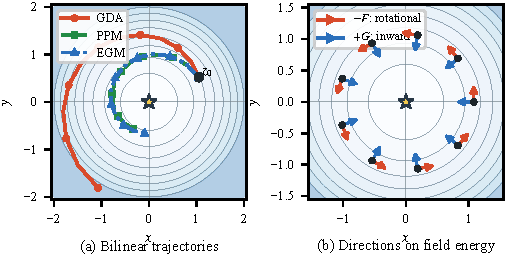
\includegraphics[width=0.54\columnwidth]{figures/mathematical_motivation.pdf}
\caption{Why saddle-field step sizes must adapt to local coupling.
For the local update $\bz_+=\bz-\beta\bF_\omega(\bz)+\gamma\nabla\bF_\omega(\bz)\bF_\omega(\bz)$, $\omega$ denotes coupling strength, $\beta$ and $\gamma$ are the field and curvature step sizes, and $q=\|\bz_+\|/\|\bz\|$ is the one-step norm ratio.
Panels (a) and (b) show the rotational field action and inward Jacobian--field action.
Panel (c) shows that the contraction region $q<1$ and its locally minimizing curvature-to-field ratio $\gamma/\beta$ vary with $\omega$.
Panel (d) follows switching coupling: a fixed ratio crosses $q=1$, whereas the local ratio remains contractive.}
\label{fig:motivation}
\end{figure}

A two-player zero-sum Markov game captures this interaction \cite{Shapley1953StochasticGames,Littman1994MarkovGames}.
The transmitter policy $\pi_{\btheta}$, with parameter vector $\btheta$, maximizes a discounted spectral-efficiency return, while the jammer policy $\nu_{\bpsi}$, with parameter vector $\bpsi$, minimizes it through $\max_{\btheta}\min_{\bpsi}J(\btheta,\bpsi)$.
Their policy gradients form a saddle field; worst-case transmitter return measures communication robustness, while exploitability measures sensitivity to further policy adaptation.

Fig.~\ref{fig:motivation} isolates the resulting learning mechanism.
In a bilinear local model, simultaneous gradient descent--ascent (GDA) follows a rotational field action and can cycle, while the Jacobian--field action supplies radial contraction \cite{Balduzzi2018Mechanics}.
The contraction region depends on both local coupling and the field-to-curvature step-size ratio; when the wireless state or either neural policy changes that coupling, a fixed ratio can move from contraction to expansion.
The proximal point method (PPM) evaluates the field implicitly, whereas the extragradient method (EGM) uses an extrapolated pair \cite{Rockafellar1976PPM,Korpelevich1976Extragradient}.
Their local expansions include a Jacobian--field action but couple the effective field and curvature scales through one learning rate \cite{Lu2022ODE}.
Adaptive Mirror-Prox methods use observed operator geometry to tune extragradient updates across smoothness regimes \cite{Antonakopoulos2021AdaProx}, while double-step extragradient assigns distinct scales to the extrapolation and update stages \cite{Hsieh2020DSEG}.
Our formulation instead treats the policy-gradient field and its Jacobian--field correction as separate search coordinates whose local coupling changes with the wireless state and neural policies.

Field-energy reduction alone does not ensure a useful communication policy.
Motivated by adaptive learning-rate and Lyapunov-drift control \cite{Zhang2025AdaptivePolyak,Yuan2025StepSizeSDE}, we therefore use the predicted one-step change of a communication-aware Lyapunov merit to coordinate geometric stabilization, worst-case-rate loss, and exploitability.

In this paper, we develop Lyapunov-Controlled Minimax Policy Learning (LCMPL) for adaptive anti-jamming DSA.
LCMPL assigns separate step sizes to the joint policy-gradient field and its Jacobian--field correction by minimizing a local model of this change.
A box-constrained quadratic model proposes both step sizes, and a same-state safeguard retains curvature only when it does not worsen realized merit or worst-case rate relative to the field-only candidate.
We prove an $O(1/K)$ stationarity transient with an interpretable residual and, under a local policy-gap condition, bound worst-case-rate loss.

\section{Adversarial DSA System and Markov-Game Model}
\subsection{Multi-Channel Wireless Environment and Stage Utility}
\begin{figure}[t]
\centering
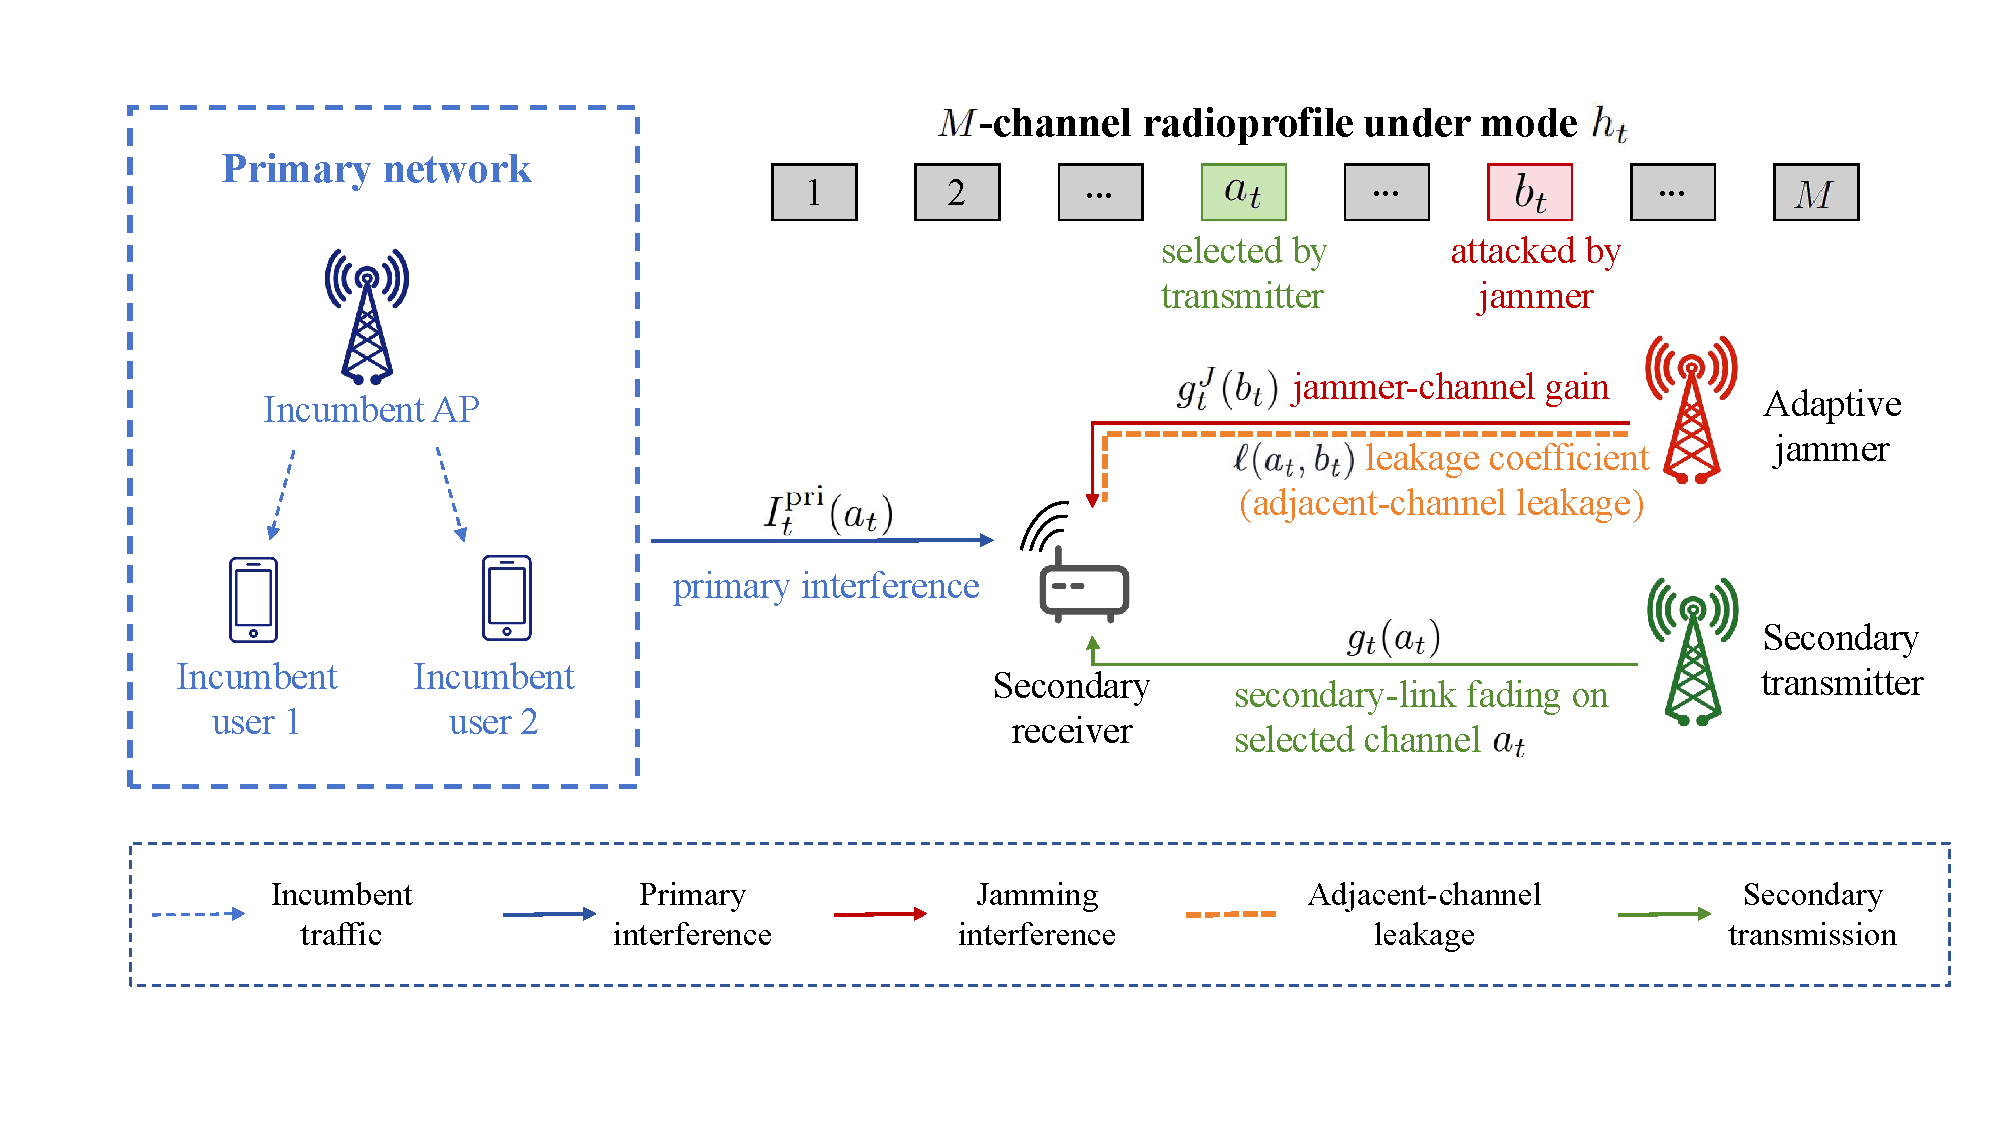
\includegraphics[width=0.68\columnwidth, trim=40 65 0 30, clip]{figures/system_model.pdf}
\caption{Adversarial wireless environment for anti-jamming dynamic spectrum access.}
\label{fig:system}
\end{figure}

Fig.~\ref{fig:system} shows an incumbent network, a secondary link, and an adaptive jammer over $M$ licensed subchannels.
The discrete variable $h_t\in\mathcal H=\{1,\ldots,L\}$ labels the current channel-occupancy or radio mode.
It is neither a selected channel nor a scalar gain; it indexes the complete channel-condition profile that applies at time $t$.
Conditional on this mode, $g_t(a)$ is the secondary-link gain on channel $a$, while $I_t$ collects the incumbent-interference profile $I_t^{\rm pri}(a)$ and jammer--receiver gains $g_t^J(b)$.
The transmitter and jammer simultaneously choose channels $a_t\in\cA$ and $b_t\in\cB$, where $\cA=\cB=\{0,\ldots,M-1\}$.
The observed Markov state is $s_t=(h_t,g_t,I_t,a_{t-1})\in\cS$; the previous transmitter channel $a_{t-1}$ is included because changing channels incurs a switching cost.
In the reported finite benchmark, the background interference and jammer--receiver gain are fixed, and each mode $h_t$ selects a distinct secondary-link gain vector $g(h_t)$.
Consequently, $g(h_t)$ together with one-hot $a_{t-1}$ gives both neural policies a one-to-one encoding of the $LM$ compact states.

The constants $P_{\rm s}$, $P_{\rm J}$, and $N_0$ denote secondary transmission power, jammer interference level, and receiver noise power, respectively.
The factor $\ell(a,b)$ models co-channel, adjacent-channel, and nonadjacent leakage, and $c_{\rm sw}\geq0$ is the switching cost.
For actions $(a_t,b_t)$, the received signal-to-interference-plus-noise ratio (SINR) and switching-cost-adjusted stage spectral efficiency are
\begin{equation}
\begin{aligned}
\operatorname{SINR}_t
&=\frac{P_{\rm s}g_t(a_t)}{N_0+I_t^{\rm pri}(a_t)+P_{\rm J}g_t^J(b_t)\ell(a_t,b_t)},\\
r_t
&=\log_2(1+\operatorname{SINR}_t)-c_{\rm sw}\mathbf 1_{\{a_t\neq a_{t-1}\}}.
\end{aligned}
\label{eq:reward}
\end{equation}
Here, $\mathbf 1_{\{\cdot\}}$ is the indicator function.
\subsection{Radio Dynamics and Minimax Policy Objective}
The radio mode follows an action-independent correlated Markov chain with transition matrix $P_h$, and the compact benchmark transition is
\[
P\big((h',a')\mid(h,a_{\rm prev}),a,b\big)
=P_h(h'|h)\mathbf 1_{\{a'=a\}}.
\]
We use $P_h(h|h)=\rho_h$ and $P_h(h'|h)=(1-\rho_h)/(L-1)$ for $h'\ne h$, where $\rho_h$ controls temporal correlation.
The reported benchmarks set $L=M$ and initialize uniformly over the $LM$ compact states.
This specialization makes the exogenous chain control correlated secondary-link fading, while the adaptive jammer creates endogenous interference through its selected channel and leakage profile.
The wireless model above specifies the physical interaction.
We next define the learning objective and distinguish it from the communication quantity used for evaluation.
Let $\pi_{\btheta}(a|s)$ and $\nu_{\bpsi}(b|s)$ denote differentiable transmitter and jammer policies.
The physical normalized discounted spectral-efficiency return is
\[
J(\btheta,\bpsi)=(1-\delta)\E\!\left[\sum_{t=0}^{\infty}\delta^t r_t\right],
\]
where $\delta\in(0,1)$ is the discount factor.
Policy-gradient training can concentrate either softmax policy early and suppress exploration as the radio mode or opponent changes.
We therefore train with the entropy-regularized return
\[
J_\tau=J+(1-\delta)\tau\E\!\left[\sum_{t\geq0}\delta^t\{H(\pi_{\btheta}(\cdot|s_t))-H(\nu_{\bpsi}(\cdot|s_t))\}\right],
\]
where $\tau>0$ is the entropy weight and $H(\cdot)$ is the Shannon entropy.
The entropy terms preserve exploration and smooth the best-response quantities used by the controller.
Policy gradients and the merit use $J_\tau$, whereas the rate safeguard and reported rates use $J$ and retain their physical bit/s/Hz meaning.
To test robustness beyond the current neural opponent, let $\Pi_{\rm T}$ and $\Pi_{\rm J}$ be the full stationary Markov policy spaces.
The primary metric is the learned transmitter's worst-case return over $\Pi_{\rm J}$,
\[
R_{\rm BR}(\btheta)=\min_{\nu\in\Pi_{\rm J}}J(\pi_{\btheta},\nu).
\]
The unregularized exploitability diagnostic measures the remaining improvement available to either player:
\[
\Delta(\bz)=\max_{\pi\in\Pi_{\rm T}}J(\pi,\nu_{\bpsi})-\min_{\nu\in\Pi_{\rm J}}J(\pi_{\btheta},\nu).
\]
Replacing $J$ by $J_\tau$ defines the smooth regularized gap $\Delta_\tau$ used only inside the training merit.
Dynamic programming computes $R_{\rm BR}$, $\Delta$, and its soft counterpart $\Delta_\tau$.
With the communication objective fixed, the next section addresses the instability of simultaneous transmitter--jammer adaptation.

\section{Geometry-Aware Minimax Policy Learning}
\subsection{Curvature-Induced Two-Direction Learning}
For the joint parameter $\bz=(\btheta,\bpsi)$, define the saddle field
\begin{equation}
\bF(\bz)=
\begin{bmatrix}
-\nabla_{\btheta}J_\tau(\btheta,\bpsi)\\
\nabla_{\bpsi}J_\tau(\btheta,\bpsi)
\end{bmatrix}.
\label{eq:field}
\end{equation}
For a learning rate $s>0$, $\bz_+=\bz-s\bF(\bz)$ ascends in the transmitter policy and descends in the jammer policy, while either update changes the opponent's gradient.
We assess GDA through the field energy $\phi(\bz)=\norm{\bF(\bz)}^2/2$, a scaled squared stationarity residual.
For GDA, $\phi(\bz-s\bF)=\phi(\bz)-s\langle\nabla\phi,\bF\rangle+O(s^2)$.
The first-order decrease can vanish when the transmitter--jammer Jacobian is dominated by its antisymmetric component, allowing GDA to rotate while $\bF$ remains nonzero.
PPM and EGM respond to this field variation by evaluating the field after a policy displacement:
\[
\begin{aligned}
\textnormal{GDA:}\quad &\bz_{+}^{\rm GDA}=\bz-s\bF(\bz),\\
\textnormal{PPM:}\quad &\bz_{+}^{\rm PPM}=\bz-s\bF(\bz_{+}^{\rm PPM}),\\
\textnormal{EGM:}\quad &\widetilde{\bz}=\bz-s\bF(\bz),\quad
\bz_{+}^{\rm EGM}=\bz-s\bF(\widetilde{\bz}),
\end{aligned}
\]
Here, $\widetilde{\bz}$ is EGM's extrapolation point; PPM uses an implicit next-policy gradient, while EGM uses an explicit predictor.
Let $\nabla\bF(\bz)$ denote the Jacobian of the saddle field.
Expanding the displaced field in EGM, or the implicit field in PPM, gives $\bz_+=\bz-s\bF(\bz)+s^2\nabla\bF(\bz)\bF(\bz)+O(s^3)$.
Their common correction motivates the Jacobian--field direction
\begin{equation}
\bG(\bz)=\nabla\bF(\bz)\bF(\bz).
\label{eq:g_direction}
\end{equation}
Thus, $\bG$ predicts how simultaneous transmitter--jammer movement changes the next joint policy gradient; Section~IV identifies when it counters rotational coupling.
Their second-order expansions couple the field and curvature terms through the fixed relation $(s,s^2)$.
Because the geometry can change independently along these directions, LCMPL assigns field and curvature step sizes $\beta_k$ and $\gamma_k$:
\begin{equation}
\bz_{k+1}=\bz_k-\beta_k\widehat{\bF}_k+\gamma_k\widehat{\bG}_k.
\label{eq:update}
\end{equation}
Here, $\widehat{\bF}_k$ and $\widehat{\bG}_k$ are stochastic oracles for $\bF(\bz_k)$ and $\bG(\bz_k)$, respectively.
In the trajectory-sampled realization, the same batch defines the empirical field and the Jacobian--vector product (JVP)
\[
\widehat{\bG}_k=\nabla\widehat{\bF}_k(\bz_k)\widehat{\bF}_k(\bz_k).
\]
The biased-oracle model in Section~IV accounts for the resulting same-batch JVP error.
The curvature direction introduces no additional wireless action; it modifies only the policy update using local game geometry.
The remaining design problem is to choose $\beta_k$ and $\gamma_k$ without trading policy stabilization for communication performance.

\subsection{Communication-Aware Lyapunov Policy Update}
Because field energy measures stationarity rather than communication quality, LCMPL evaluates both directions through a Lyapunov merit combining field energy, exploitability, and worst-case-rate deficit.
Define the normalized communication loss
\[
\mathcal L_{\rm c}(\bz)=
\lambda_\Delta\left(\frac{\Delta_\tau(\bz)}{\Delta_{\tau,0}}\right)^2
+\lambda_R\left(\frac{D_{R,\tau}(\btheta)}{D_0}\right)^2,
\]
where $\lambda_\Delta,\lambda_R\geq0$ are merit weights and $\Delta_{\tau,0},D_0>0$ are initial scales.
Let $r_{\max}$ be the largest stage reward in the finite game and define the entropy-regularized stage-return ceiling $R_{{\rm ub},\tau}=r_{\max}+\tau\log M$.
The deficit $D_{R,\tau}=R_{{\rm ub},\tau}-\min_{\nu\in\Pi_{\rm J}}J_\tau(\pi_{\btheta},\nu)\geq0$ uses this ceiling for normalization.
The Lyapunov merit is
\begin{equation}
V(\bz)=\frac{\phi(\bz)}{\phi_0}+\mathcal L_{\rm c}(\bz),
\label{eq:merit}
\end{equation}
where $\phi_0>0$ is the initial field-energy scale.
The merit is a training control signal, not a replacement for the reported physical rate.
Its predicted one-step change supplies a common criterion for geometric stabilization and communication quality.

The update in Eq.~\eqref{eq:update} lies in a two-dimensional span even when the neural parameter space is large.
LCMPL therefore models the merit only along the sampled field and curvature directions, avoiding a full parameter-space Hessian.
Let $\bd_{k,1}=-\widehat{\bF}_k$, $\bd_{k,2}=\widehat{\bG}_k$, and let $\bu=(\beta,\gamma)^{\mathsf T}$ collect their candidate step sizes.
For positive probe radii $\varepsilon_{k,1}$ and $\varepsilon_{k,2}$, evaluate $V_{k,i}^{\pm}=V(\bz_k\pm\varepsilon_{k,i}\bd_{k,i})$ and $V_k^0=V(\bz_k)$.
Centered finite differences estimate the first and second directional changes as $[\ba_k]_i=(V_{k,i}^{+}-V_{k,i}^{-})/(2\varepsilon_{k,i})$ and
\[
[\bH_k]_{ii}=\max\!\left\{\frac{V_{k,i}^{+}-2V_k^0+V_{k,i}^{-}}{\varepsilon_{k,i}^2},h_{\min}\right\}
\]
for $i\in\{1,2\}$, with $[\bH_k]_{12}=[\bH_k]_{21}=0$ and $h_{\min}>0$.
The positive floor $h_{\min}$ makes each scalar model well posed, and the diagonal form avoids mixed-direction probes.
If $\widehat{\bG}_k=0$, set $[\ba_k]_2=0$ and $[\bH_k]_{22}=h_{\min}$; the QP then reduces to the field-only model.
Let $\bar\beta>0$ and $0<\gamma_{\min}\leq\gamma_{\max}$ be deterministic global step-size bounds, and let the oracle-dependent cap $\gamma_{\min}\leq\bar\gamma_k\leq\gamma_{\max}$ be measurable after the current oracle query.
LCMPL selects the two step sizes with the box-constrained quadratic program (QP)
\begin{equation}
\begin{aligned}
m_k(\bu)&=\ba_k^{\mathsf T}\bu+\tfrac12\bu^{\mathsf T}\bH_k\bu,\\
\widetilde{\bu}_k&=\operatorname*{arg\,min}_{\bu\in\mathcal U_k}m_k(\bu),
\quad
\mathcal U_k=[0,\bar\beta]\times[0,\bar\gamma_k].
\end{aligned}
\label{eq:boxqp}
\end{equation}
Let $\bu_k^F$ minimize $m_k$ over $\mathcal U_F=[0,\bar\beta]\times\{0\}$.
Define the extra fitted-model decrease supplied by the curvature coordinate as $D_{G,k}^{\rm box}=m_k(\bu_k^F)-m_k(\widetilde{\bu}_k)\geq0$.
Because the local model need not predict a finite step exactly, LCMPL backtracks $\widetilde{\bu}_k$ and $\bu_k^F$ independently from the same $\bz_k$ until the realized merit does not increase; a failed search returns zero.
Denote the backtracked pairs by $\bar{\bu}_k$ and $\bar{\bu}_k^F$.
The safeguard accepts $\bu_k^{\rm acc}=\bar{\bu}_k$ when it has no larger realized $V$ and no smaller $R_{\rm BR}$ than $\bar{\bu}_k^F$; otherwise, it selects $\bar{\bu}_k^F$ and uses $(\beta_k,\gamma_k)^{\mathsf T}=\bu_k^{\rm acc}$ in Eq.~\eqref{eq:update}.
LCMPL-F fixes $\gamma_k=0$ while retaining the field-direction merit, probes, QP, and safeguard.
Fig.~\ref{fig:framework} summarizes the loop in which communication feedback forms a trajectory batch $\mathcal B_k$ for the field and Jacobian-action estimates.

\begin{figure}[t]
\centering
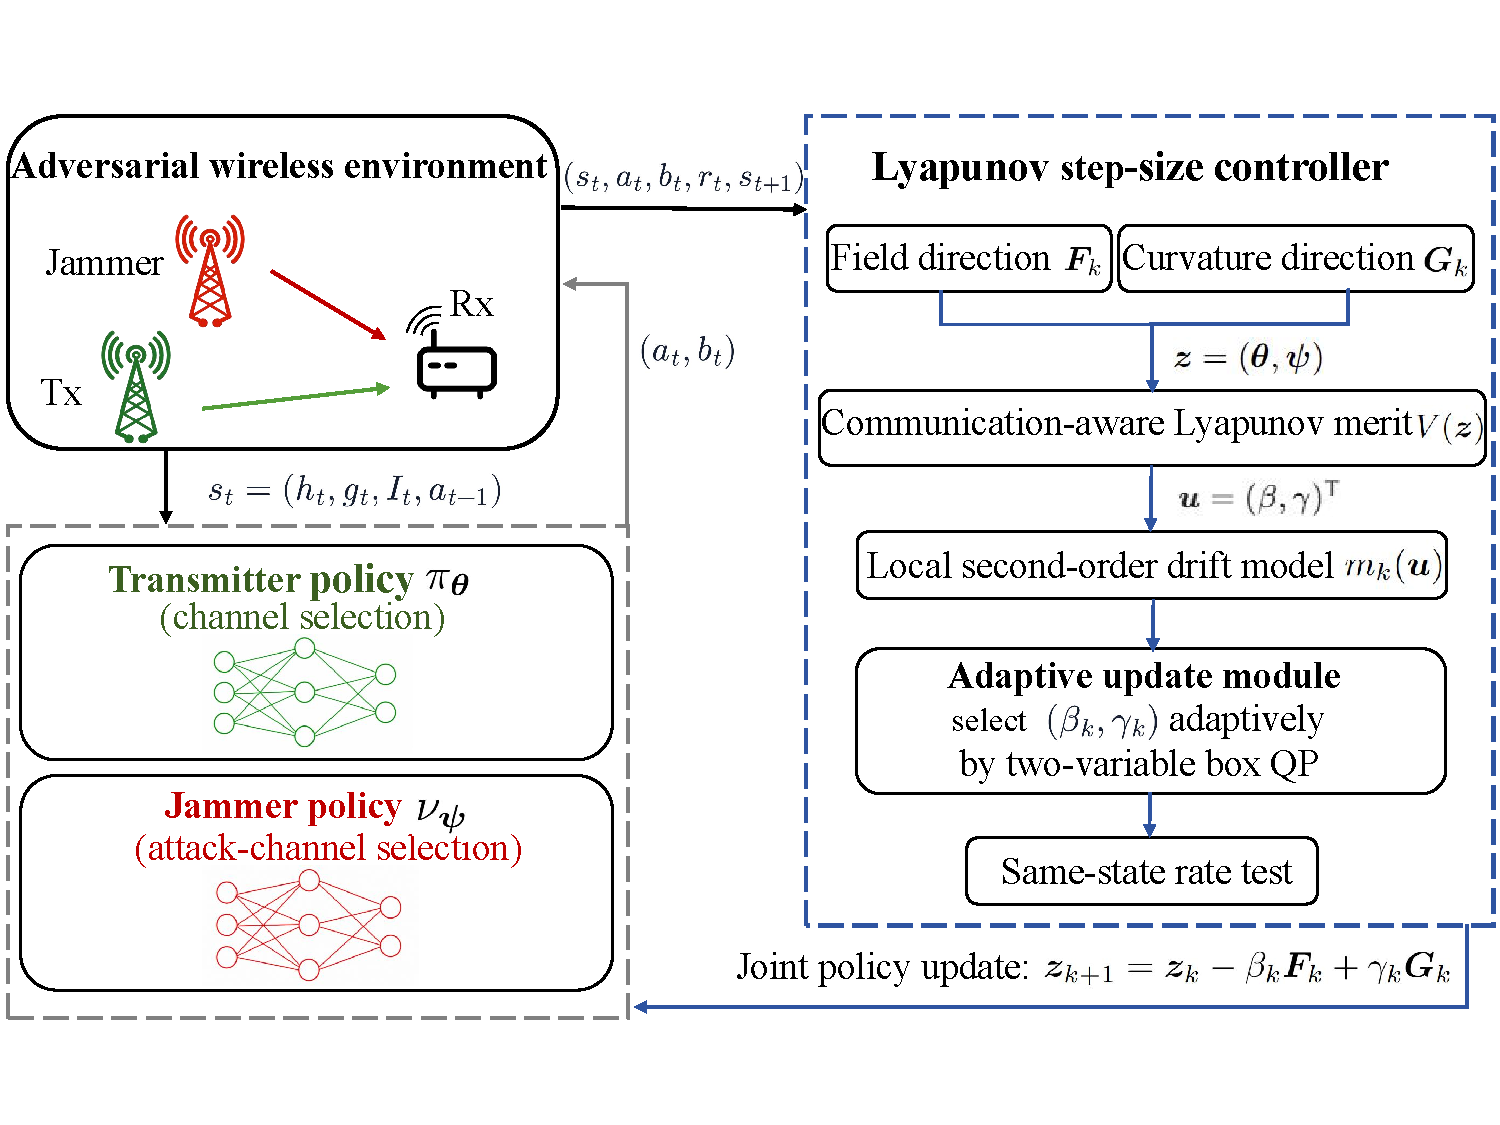
\includegraphics[width=0.68\columnwidth, trim=50 65 40 30, clip]{figures/algorithm_framework.pdf}
\caption{LCMPL minimax policy-learning framework.}
\label{fig:framework}
\end{figure}

\section{Learning Stability and Communication Guarantees}
The analysis first determines when $+\bG$ decreases field energy, then connects the accepted decrease in the local Lyapunov model to finite-time communication performance.
Write $\nabla\bF=\bS+\bW$, where $\bS=(\nabla\bF+\nabla\bF^{\mathsf T})/2$ and $\bW=(\nabla\bF-\nabla\bF^{\mathsf T})/2$.

\begin{proposition}[Curvature identity for adversarial policy learning]
\label{prop:curvature}
At every point where $\bF$ is differentiable, the Jacobian--field direction satisfies
\begin{equation}
\langle\nabla\phi,\bG\rangle=\norm{\bS\bF}^2-\norm{\bW\bF}^2.
\label{eq:skew_identity}
\end{equation}
Hence, $+\bG$ decreases the field energy when $\norm{\bW\bF}>\norm{\bS\bF}$.
\end{proposition}

\emph{Proof:}
With $\bA=\nabla\bF$, $\langle\nabla\phi,\bG\rangle=\bF^{\mathsf T}\bA^2\bF$.
Expanding $\bA=\bS+\bW$ eliminates the cross term because $\bS\bW+\bW\bS$ is antisymmetric.
Moreover, $\bF^{\mathsf T}\bS^2\bF=\|\bS\bF\|^2$ and $\bF^{\mathsf T}\bW^2\bF=-\|\bW\bF\|^2$, which gives Eq.~\eqref{eq:skew_identity}.
\hfill$\square$

Proposition~\ref{prop:curvature} gives a deterministic geometric condition for curvature stabilization, whereas LCMPL uses stochastic field estimates and finite-difference merit probes.
We therefore separate estimation errors from geometric Lyapunov conditions.
Let $\mathcal F_k$ denote the history available immediately before drawing the stochastic-oracle and probe samples at update $k$.
The analysis starts from an explicit biased-oracle model.
\begin{assumption}[Local regularity and stochastic oracles]
\label{ass:oracles}
\begin{enumerate}
\item[(a)] A compact set $\mathcal T$ contains all accepted iterates, trial segments, and probe points, and $\bF\in C^1$ and $V\in C^3$ near $\mathcal T$, with $\|\nabla V\|\leq G_V$, $\|\nabla^2V\|\leq H_V$, and $\|\nabla^3V\|\leq M_3$.
\item[(b)] For $X\in\{F,G\}$, $\widehat{\boldsymbol X}_k=\boldsymbol X(\bz_k)+\bb_k^X+\boldsymbol\zeta_k^X$, where $\bb_k^X$ is $\mathcal F_k$-measurable and $\E[\boldsymbol\zeta_k^X\mid\mathcal F_k]=0$.
\item[(c)] Finite nonnegative $\mathcal F_k$-measurable bounds satisfy $\|\bb_k^X\|\leq b_{X,k}$ and $\E[\|\boldsymbol\zeta_k^X\|^p\mid\mathcal F_k]\leq\sigma_{p,X,k}^p$ for $p\in\{2,3\}$ and $X\in\{F,G\}$.
\end{enumerate}
\end{assumption}
The same-batch JVP error is allowed in $\bb_k^G$ and is not assumed unbiased.

Define the population field-energy decrease signals
\[
\chi_F(\bz)=\bF^{\mathsf T}\bS\bF,
\quad
\chi_G(\bz)=-\langle\nabla\phi(\bz),\bG(\bz)\rangle.
\]
Positive $\chi_F$ and $\chi_G$ certify decrease of $\phi$ along $-\bF$ and $+\bG$, respectively.
\begin{assumption}[Geometric coverage]
\label{ass:geometry}
The local coverage modulus
\begin{equation}
m_{\rm geo}
=\inf_{\substack{\bz\in\mathcal T\\\norm{\bF(\bz)}>0}}
\frac{\max\{\chi_F(\bz),\chi_G(\bz)\}}{\norm{\bF(\bz)}^2}
\label{eq:coverage}
\end{equation}
satisfies $m_{\rm geo}>0$.
\end{assumption}
Let $\sigma_{\min}$ denote the smallest singular value.
At a target stationary point $\bz^\star$, the conditions $\bS(\bz^\star)\succeq0$ and $\sigma_{\min}(\nabla\bF(\bz^\star))>0$ imply Eq.~\eqref{eq:coverage} on a sufficiently small neighborhood by compactness of the unit sphere and continuity; this includes nonsingular pure rotation, where $\chi_F=0$ and $\chi_G>0$.
Define $D_F=\langle\nabla V,\bF\rangle$ and $D_G=-\langle\nabla V,\bG\rangle$.
Compactness and smoothness make
\[
B_{\rm c}=\sup_{\bz\in\mathcal T}
\max\{\lvert\langle\nabla\mathcal L_{\rm c},\bF\rangle\rvert,
\lvert\langle\nabla\mathcal L_{\rm c},\bG\rangle\rvert\}<\infty.
\]
Because $V=\phi/\phi_0+\mathcal L_{\rm c}$, selecting the larger energy signal gives
\begin{equation}
\begin{aligned}
\max\{D_F(\bz),D_G(\bz)\}
&\geq\mu_{\rm geo}\norm{\bF(\bz)}^2-B_{\rm c},\\
\mu_{\rm geo}&=m_{\rm geo}/\phi_0.
\end{aligned}
\label{eq:geometry_certificate}
\end{equation}

The stochastic theorem separates geometric decrease from sampled-oracle and finite-probe errors.
Let $s\in(0,\min\{\bar\beta,\gamma_{\min}\}]$ be a deterministic pure-coordinate comparator, and assume bounded probe radii.
For $p\in\{2,3\}$, define $M_{p,X,k}=\E[\|\widehat{\boldsymbol X}_k\|^p\mid\mathcal F_k]$, $M_{p,k}=\max_X M_{p,X,k}$, $b_k=\max_X b_{X,k}$, and $C_{2,k}=\sqrt{M_{2,F,k}M_{2,G,k}}$.
Let $A_k=\E[m_k(\bu_k^{\rm acc})-m_k(\widetilde{\bu}_k)\mid\mathcal F_k]\geq0$ denote accepted-step model loss.
Smoothness and centered-probe bounds yield
\begin{equation}
\mathcal R_k(s)=s(G_Vb_k+B_{\rm c})
+C_s(1+M_{2,k}+M_{3,k}+C_{2,k})+A_k,
\label{eq:residual}
\end{equation}
where $C_s<\infty$ is deterministic and depends only on $s$, the smoothness constants, probe bounds, step-size box, and $h_{\min}$.
The terms in Eq.~\eqref{eq:residual} cover communication-merit variation, oracle bias and noise, probe and Taylor errors, omitted mixed curvature, and safeguard or backtracking loss.

\begin{figure*}[t]
\centering
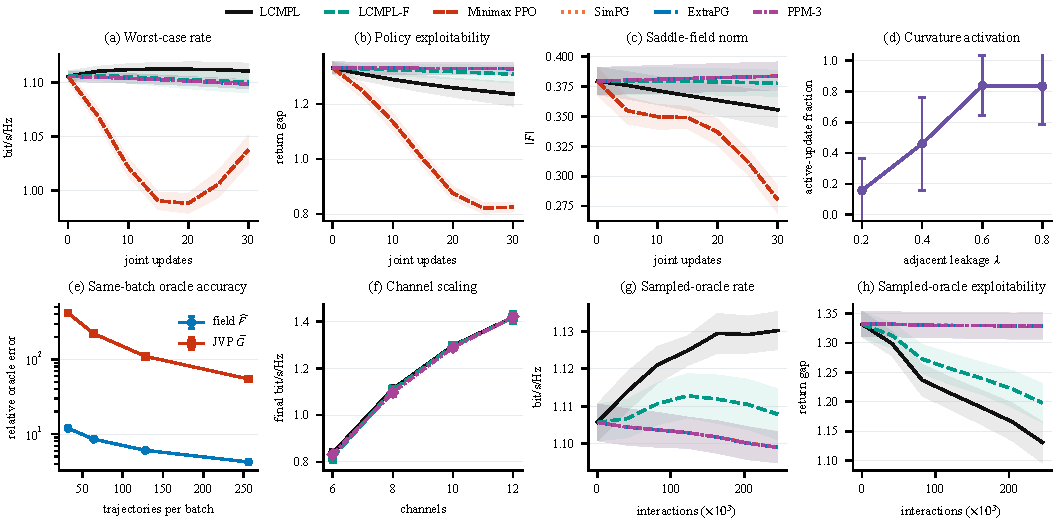
\includegraphics[width=0.63\textwidth]{results/theory_aligned_v1_20260813/figures/neural_benchmark_theory.pdf}
\caption{Adversarial DSA results: (a)--(c) nominal population dynamics; (d) leakage-dependent curvature activation; (e) oracle fidelity; (f) channel scaling; and (g)--(h) equal-interaction trajectory learning.
Means use 12 seeds except eight in (f); bands in (a)--(c) and (g)--(h) show one standard error, and bars in (d)--(f) show 95\% confidence intervals.}
\label{fig:neural}
\end{figure*}

\begin{proposition}[Conditional Lyapunov drift]
\label{prop:drift}
Under Assumptions~\ref{ass:oracles}--\ref{ass:geometry}, the implemented accepted update satisfies
\[
\begin{aligned}
&\E[V(\bz_{k+1})-V(\bz_k)\mid\mathcal F_k]\\
&\leq-s\mu_{\rm geo}\norm{\bF(\bz_k)}^2
+\mathcal R_k(s).
\end{aligned}
\]
\end{proposition}

\emph{Proof:}
At update $k$, select the larger of $D_F(\bz_k)$ and $D_G(\bz_k)$ only for the analysis.
Because both pure-coordinate pairs $(s,0)$ and $(0,s)$ are box feasible, the fitted QP decrease dominates the selected comparator.
Taylor expansion adds the probe, cubic, safeguard, and omitted mixed-Hessian residuals bounded in Eq.~\eqref{eq:residual}.
Conditional expectation removes the zero-mean errors, bounds the remaining oracle terms by their moments, and Eq.~\eqref{eq:geometry_certificate} supplies the population decrease.
\hfill$\square$

\begin{theorem}[Main finite-time minimax stationarity result]
\label{thm:stationarity}
Under Assumptions~\ref{ass:oracles}--\ref{ass:geometry}, every integer $K\geq1$ satisfies
\begin{equation}
\frac1K\sum_{k=0}^{K-1}\E\norm{\bF(\bz_k)}^2
\leq
\frac{V(\bz_0)}{s\mu_{\rm geo}K}
+\frac{\overline{\mathcal R}_K(s)}{s\mu_{\rm geo}},
\label{eq:rate}
\end{equation}
where $\overline{\mathcal R}_K=K^{-1}\sum_{k=0}^{K-1}\E\mathcal R_k$.
\end{theorem}

\emph{Proof:}
Take total expectations in Proposition~\ref{prop:drift}, sum over $k$, and use $V(\bz_K)\geq0$.
\hfill$\square$

If $\sup_k\E\mathcal R_k(s)\leq\bar R<\infty$, Theorem~\ref{thm:stationarity} gives an $O(1/K)$ transient plus the floor $\bar R/(s\mu_{\rm geo})$.
The result covers pure rotation, where the field coordinate has zero first-order effect and the curvature coordinate supplies the strict decrease predicted by Fig.~\ref{fig:motivation} and Proposition~\ref{prop:curvature}.
Here, $s$ is an analytical comparator, not an implemented learning rate.

The following local compatibility condition bridges Theorem~\ref{thm:stationarity} from neural parameter-space stationarity to full-policy best responses.

Let $v^*=\max_{\pi\in\Pi_{\rm T}}\min_{\nu\in\Pi_{\rm J}}J(\pi,\nu)$ denote the unregularized stationary-policy game value.
Since each $M$-ary policy has entropy at most $\log M$, the regularized and unregularized returns differ by at most $\tau\log M$ for either player.
Consequently,
\begin{equation}
0\leq v^*-R_{\rm BR}(\btheta)\leq\Delta_\tau(\bz)+2\tau\log M.
\label{eq:performance_bridge}
\end{equation}
Let $B_K$ denote the right-hand side of Eq.~\eqref{eq:rate}.

\begin{corollary}[Main communication result: worst-case spectral efficiency]
\label{cor:rate}
If nonnegative constants $C_{\rm gap}$ and $\xi_{\rm gap}$ satisfy $\Delta_\tau(\bz)\leq C_{\rm gap}\norm{\bF(\bz)}^2+\xi_{\rm gap}$ on $\mathcal T$, then
\[
\frac1K\sum_{k=0}^{K-1}\E\big[v^*-R_{\rm BR}(\btheta_k)\big]
\leq C_{\rm gap}B_K+\xi_{\rm gap}+2\tau\log M.
\]
\end{corollary}

\emph{Proof:}
Average Eq.~\eqref{eq:performance_bridge}, apply the local gap condition, and invoke Theorem~\ref{thm:stationarity}.
\hfill$\square$

Corollary~\ref{cor:rate} bounds worst-case spectral-efficiency loss under local compatibility between neural stationarity and the policy-space gap; the last term is the entropy-regularization error.

\begin{figure*}[t]
\centering
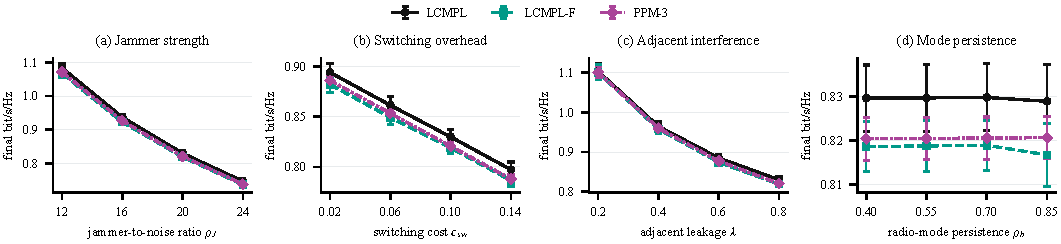
\includegraphics[width=0.68\textwidth]{results/theory_aligned_v1_20260813/figures/wireless_stress_rate.pdf}
\caption{Wireless stress across jammer strength, switching cost, leakage, and mode persistence: 12-seed means and 95\% confidence intervals.}
\label{fig:wireless_stress}
\end{figure*}

\section{Communication Performance Evaluation}
We use worst-case normalized discounted spectral-efficiency return as the primary metric and unregularized exploitability $\Delta$, field norm, and oracle error as diagnostics.
\subsection{Adversarial DSA Scenario and Evaluation Protocol}
\emph{Wireless scenario:}
We evaluate the link and adaptive jammer in Fig.~\ref{fig:system}.
The nominal benchmark uses $M=L=8$, 12 fixed seeds, $\rho_h=0.75$, $N_0=1$, $I_t^{\rm pri}(a)=0$, $g_t^J(b)=1$, $(P_{\rm s},P_{\rm J},c_{\rm sw})=(10,20,0.10)$, $\delta=0.95$, and $\tau=0.02$.
Its base secondary-link gain vector is $g_m^{\rm base}=1.9(0.18/1.9)^{m/(M-1)}$, $m=0,\ldots,M-1$, and the $L=M$ radio modes are cyclic shifts of this vector.
The jammer-to-noise ratio is $\rho_J=P_{\rm J}/N_0$ and equals 20 nominally; adjacent-channel leakage $\lambda=0.80$ enters the cyclic profile $1,\lambda,0.12,0.025$ at channel distances $0,1,2,{>}2$.
The channel-scale study uses $M=L\in\{6,8,10,12\}$, while the 12-seed wireless-stress study uses $M=L=6$ and varies $\rho_J$, $c_{\rm sw}$, $\lambda$, and $\rho_h$ one factor at a time.

\emph{Policies and comparison protocol:}
Both players use independent two-layer tanh--softmax policies with the fully observed state encoding in Section~II.
The nominal setting uses 64 hidden units, 1608 parameters per player, and 30 joint updates; stress tests use 32 units and 25 updates.
The nominal benchmark compares simultaneous policy gradient (SimPG), extragradient policy gradient (ExtraPG), a three-step PPM approximation (PPM-3), minimax proximal policy optimization (Minimax PPO), LCMPL-F, and LCMPL.
They share the environment, policies, initialization, test seeds, entropy coefficient, outer-update count, and simultaneous start without warm-up; the five saddle-field rules also share the entropy-regularized policy-gradient oracle.
Minimax PPO is a population clipped-surrogate reference with root-mean-square-normalized exact advantages and three clip-$0.2$ epochs of fresh per-update Adam~\cite{Schulman2017PPO}.
Disjoint validation seeds select rates $0.01$ for the fixed-step rules and $10^{-3}$ for Minimax PPO from prespecified grids.
LCMPL-F is the field-only ablation defined in Section~III-B.

\emph{LCMPL configuration:}
Let $f_k=\|\widehat{\bF}_k\|$ and $g_k=\|\widehat{\bG}_k\|$.
The probe radii scale inversely with $f_k$ and $g_k$ and are capped at $0.012$ and $0.025$, respectively; the released configuration records their exact rule.
We set $\bar\beta=0.08$, $\gamma_{\min}=5\times10^{-4}$, $\gamma_{\max}=0.12$, $\bar\gamma_k=\min\{\gamma_{\max},\max\{\gamma_{\min},0.08f_k/\max(g_k,10^{-12})\}\}$, and $h_{\min}=10^{-6}$; at most eight backtracking contractions by $1/2$ seek a merit change no larger than $10^{-10}$.
The merit uses weights $(\lambda_\Delta,\lambda_R)=(0.35,1.5)$, and its components are normalized by their positive initial values.

\subsection{Nominal Anti-Jamming Performance}
LCMPL's final mean worst-case rate is $1.1106$ bit/s/Hz, versus $1.1005$ for LCMPL-F, $1.0984$ for PPM-3, and $1.0380$ for Minimax PPO in Fig.~\ref{fig:neural}(a).
Its paired gains over LCMPL-F are $0.0102$ bit/s/Hz in rate with a 95\% confidence interval of $[0.0006,0.0197]$ and $0.0728$ in exploitability reduction with interval $[0.0346,0.1109]$.
Minimax PPO reaches smaller final optimization residuals but a lower rate, showing that stationarity alone does not ensure communication robustness.

\subsection{Channel Scalability and Stochastic-Oracle Fidelity}
Fig.~\ref{fig:neural}(f) shows that LCMPL exceeds LCMPL-F in final mean worst-case rate across 6--12 channels.
Panel (e) compares sampled and exact finite-game oracles at updates 0, 15, and 30 over 12 seeds using $e_X=\|\widehat{\boldsymbol{X}}-\boldsymbol{X}\|/\max\{\|\boldsymbol{X}\|,10^{-12}\}$ for $X\in\{F,G\}$.
Increasing the batch from 32 to 256 trajectories reduces mean relative field and JVP errors by $64.7\%$ and $86.9\%$, respectively.

\subsection{Trajectory-Sampled Anti-Jamming Learning}
Panels (g) and (h) test the trajectory-sampled realization in Fig.~\ref{fig:framework}.
Each update uses 128 length-64 on-policy trajectories, and every method receives 245,760 transitions per seed.
Both players share one batch; automatic differentiation forms $\widehat{\bG}_k$, while ExtraPG and PPM-3 reuse the batch through per-decision likelihood ratios.
Exact finite-game dynamic programming evaluates the merit, safeguard, and evaluation checkpoints.
At the final budget, LCMPL improves worst-case rate over LCMPL-F by $0.0223$ bit/s/Hz with a paired 95\% confidence interval of $[0.0138,0.0308]$ and reduces exploitability by $0.0672$ with interval $[0.0440,0.0903]$.
LCMPL also attains a higher rate and lower exploitability than SimPG, ExtraPG, and PPM-3.
After safeguarding, $\gamma_k>10^{-10}$ on $25.3\%$ of 360 updates, while the field-only candidate is selected on another $24.2\%$.

\subsection{Robustness Across Wireless Operating Points}
Fig.~\ref{fig:neural}(d) shows 12-seed leakage-dependent curvature activation, while Fig.~\ref{fig:wireless_stress} retrains LCMPL, LCMPL-F, and PPM-3 under one-factor changes in jammer-to-noise ratio, switching cost, leakage, and mode persistence.
LCMPL has the highest final mean rate in every plotted sweep cell, with paired mean gains of $0.0019$--$0.0161$ bit/s/Hz over LCMPL-F.

\section{Conclusion}
LCMPL separates field and curvature step sizes in adversarial DSA and retains curvature only when the same-state safeguard validates its merit and rate.
The biased-oracle analysis bounds time-averaged stationarity and, under a local policy-gap condition, worst-case spectral-efficiency loss; LCMPL achieves the highest final mean rate across the reported regimes.

\bibliographystyle{IEEEtran}
\bibliography{refs}

\end{document}
